\chapter{Conclusions}

This project explored how to utilize GPUs for photorealistic rendering. The project implemented a parallel version of the path-tracing algorithm, as well as a variant of path-tracing where online reinforcement learning guides the generation of new rays. These algorithms are accelerated by a Bounding Volume Hierarchy system, where state-of-the-art BVH construction, optimization, and traversal procedures are implemented. The project demonstrates how these different algorithms can be combined and parallelized together to form an extremely efficient photorealistic rendering system. The software created is named \texttt{Cavalry}, and its full source code is available at \url{https://github.com/AmesingFlank/Cavalry}.

\section{Limitations \& Future Work}
This section begins by listing a few of the algorithmic details of \texttt{Cavalry} that are fairly important, but were not be described in this report due to the word-count limit:
\begin{itemize}
    \item Quasi-random number generation:
    
    This project implemented a carefully designed random number generator, which has the \textit{low-discrepancy} property and is specially suited for generating random samples used by a Monte Carlo integrator. 

    \item Physically based BRDFs:
    
    In order to produce realistic images, it is vital that BRDFs of different materials be implemented in a physically correct manner. A family of BRDFs known for their physical accuracy are the Microfacet BRDFs\cite{cook1982reflectance}, which are well implemented by this project. 

\end{itemize}

\label{section limitations}
This section also lists a few valuable features that would make \texttt{Cavalry} more complete and powerful as a renderer. Even though these features not yet supported, they can be added in future endeavors.

\begin{itemize}

    \item Sub-surface scattering
    
    For most surfaces, when a light ray hits the surface at a point, the reflected rays start at the exact same point. However, this is not true for all objects in the real world. There are certain materials (e.g., jade) such that light enters the object at one point, and leaves the object at a slightly different point. These materials are described by bi-directional scattering-surface reflectance distribution functions (BSSRDFs), written as $S(p_o,w_o,p_i,w_i)$. The additional argument $p_o$ to this reflectance function brings extra complexity to the renderer, but also enables it to capture a more complete range of real world objects.

    \begin{figure}[H]
        \centering
        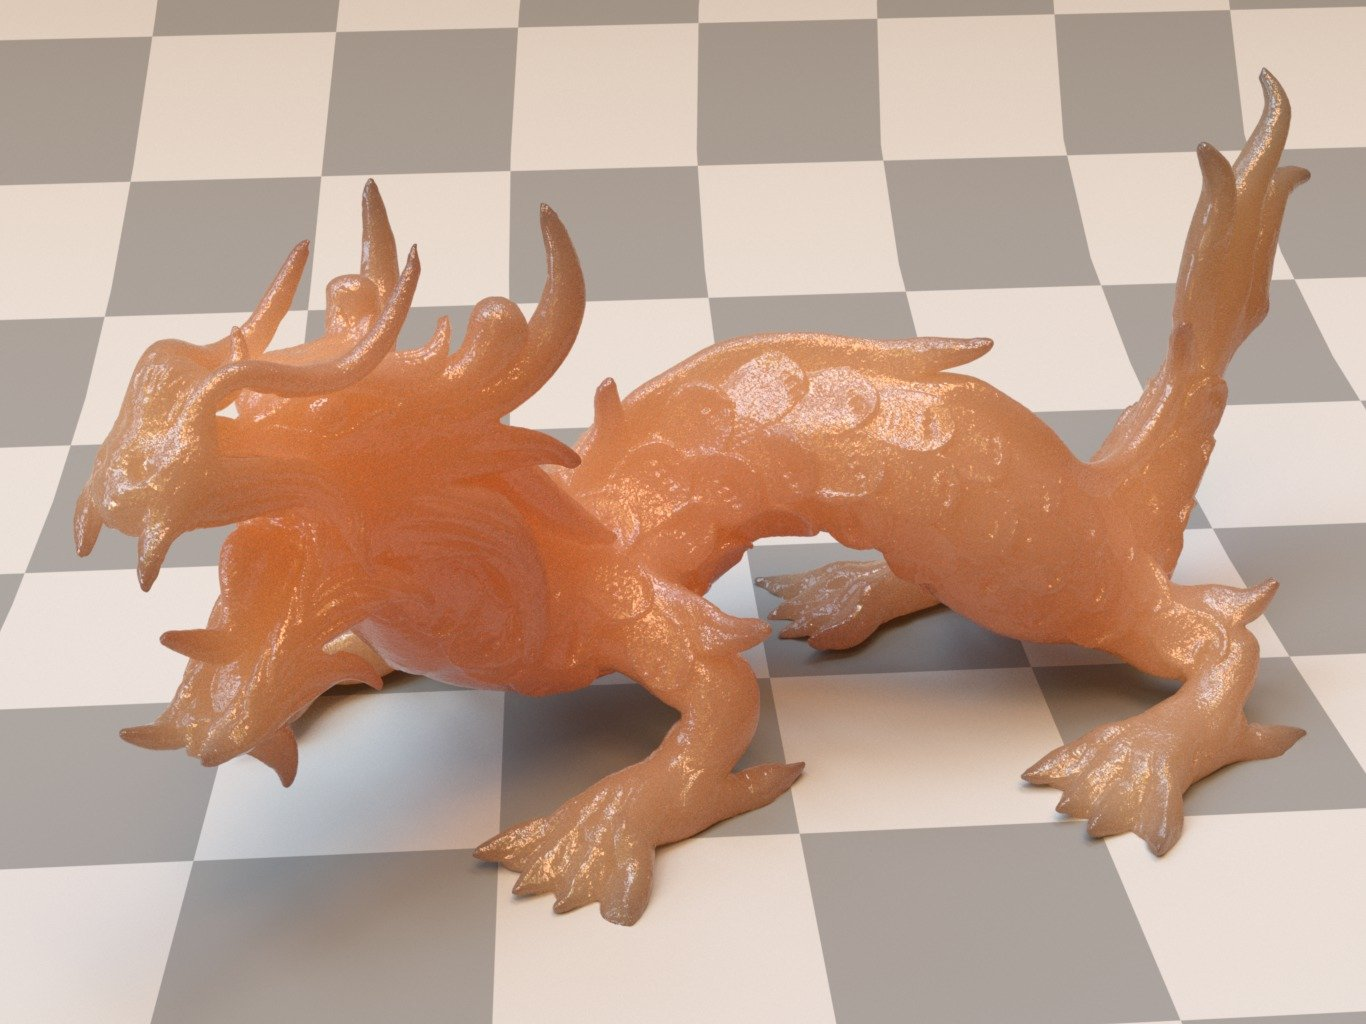
\includegraphics[height = 6cm]{dragon_10.jpg}
        \caption{Dragon model with sub-surface scattering. Rendered using \texttt{pbrt}.}
    \end{figure}

    \item Participating media
    
    In the real world, the media through which light travels can sometimes scatter, emit, or absorb light. Modelling these interactions are essential for the rendering of phenomenons such as fire and smoke. 

    

    \item Other variants of path-tracing.
    
    Apart from the reinforcement learning integrator, many other variants of path tracing exists, each with its own benefits. Two of the most powerful versions are Metropolis Light Transport, which uses a Markov chain whose stationary distribution converges to an optimal path-sampling distribution, and Gradient Domain Path-Tracing, which accelerates rendering by also estimating the difference between adjacent pixels. Implementing these algorithms would allow the \texttt{Cavalry} renderer to more robustly support a broader range of scenes.


\end{itemize}



\section{Personal Reflections}
Working on this project had been the most intensive intellectual endeavor I have made in my student career. Building the GPU renderer from scratch was a thorough training of comprehending and reproducing academic research, and it tested my abilities of organizing a complex code base. In the end, apart from the improvements mentioned in section \ref{section limitations}, which I wish I made more progress on, I am in general very happy with and proud of the outcomes of this project.

One aspect of this project that I particular enjoyed is that, because physically based rendering is an extensively studied field, there is always a plethora of papers to refer to. I particularly enjoyed comparing academic results on the same topic from different years, and seeing how peoples' understanding of a problem progresses. This processes gives me a comprehensive view of each algorithm: why does it work, what is it inspired from, and why has it been superseded by other approaches. These papers reflect just how much rendering technologies have improved over the past few decades, and it makes me excited about future developments of computer graphics.

\begin{figure}[H]
    \centering
    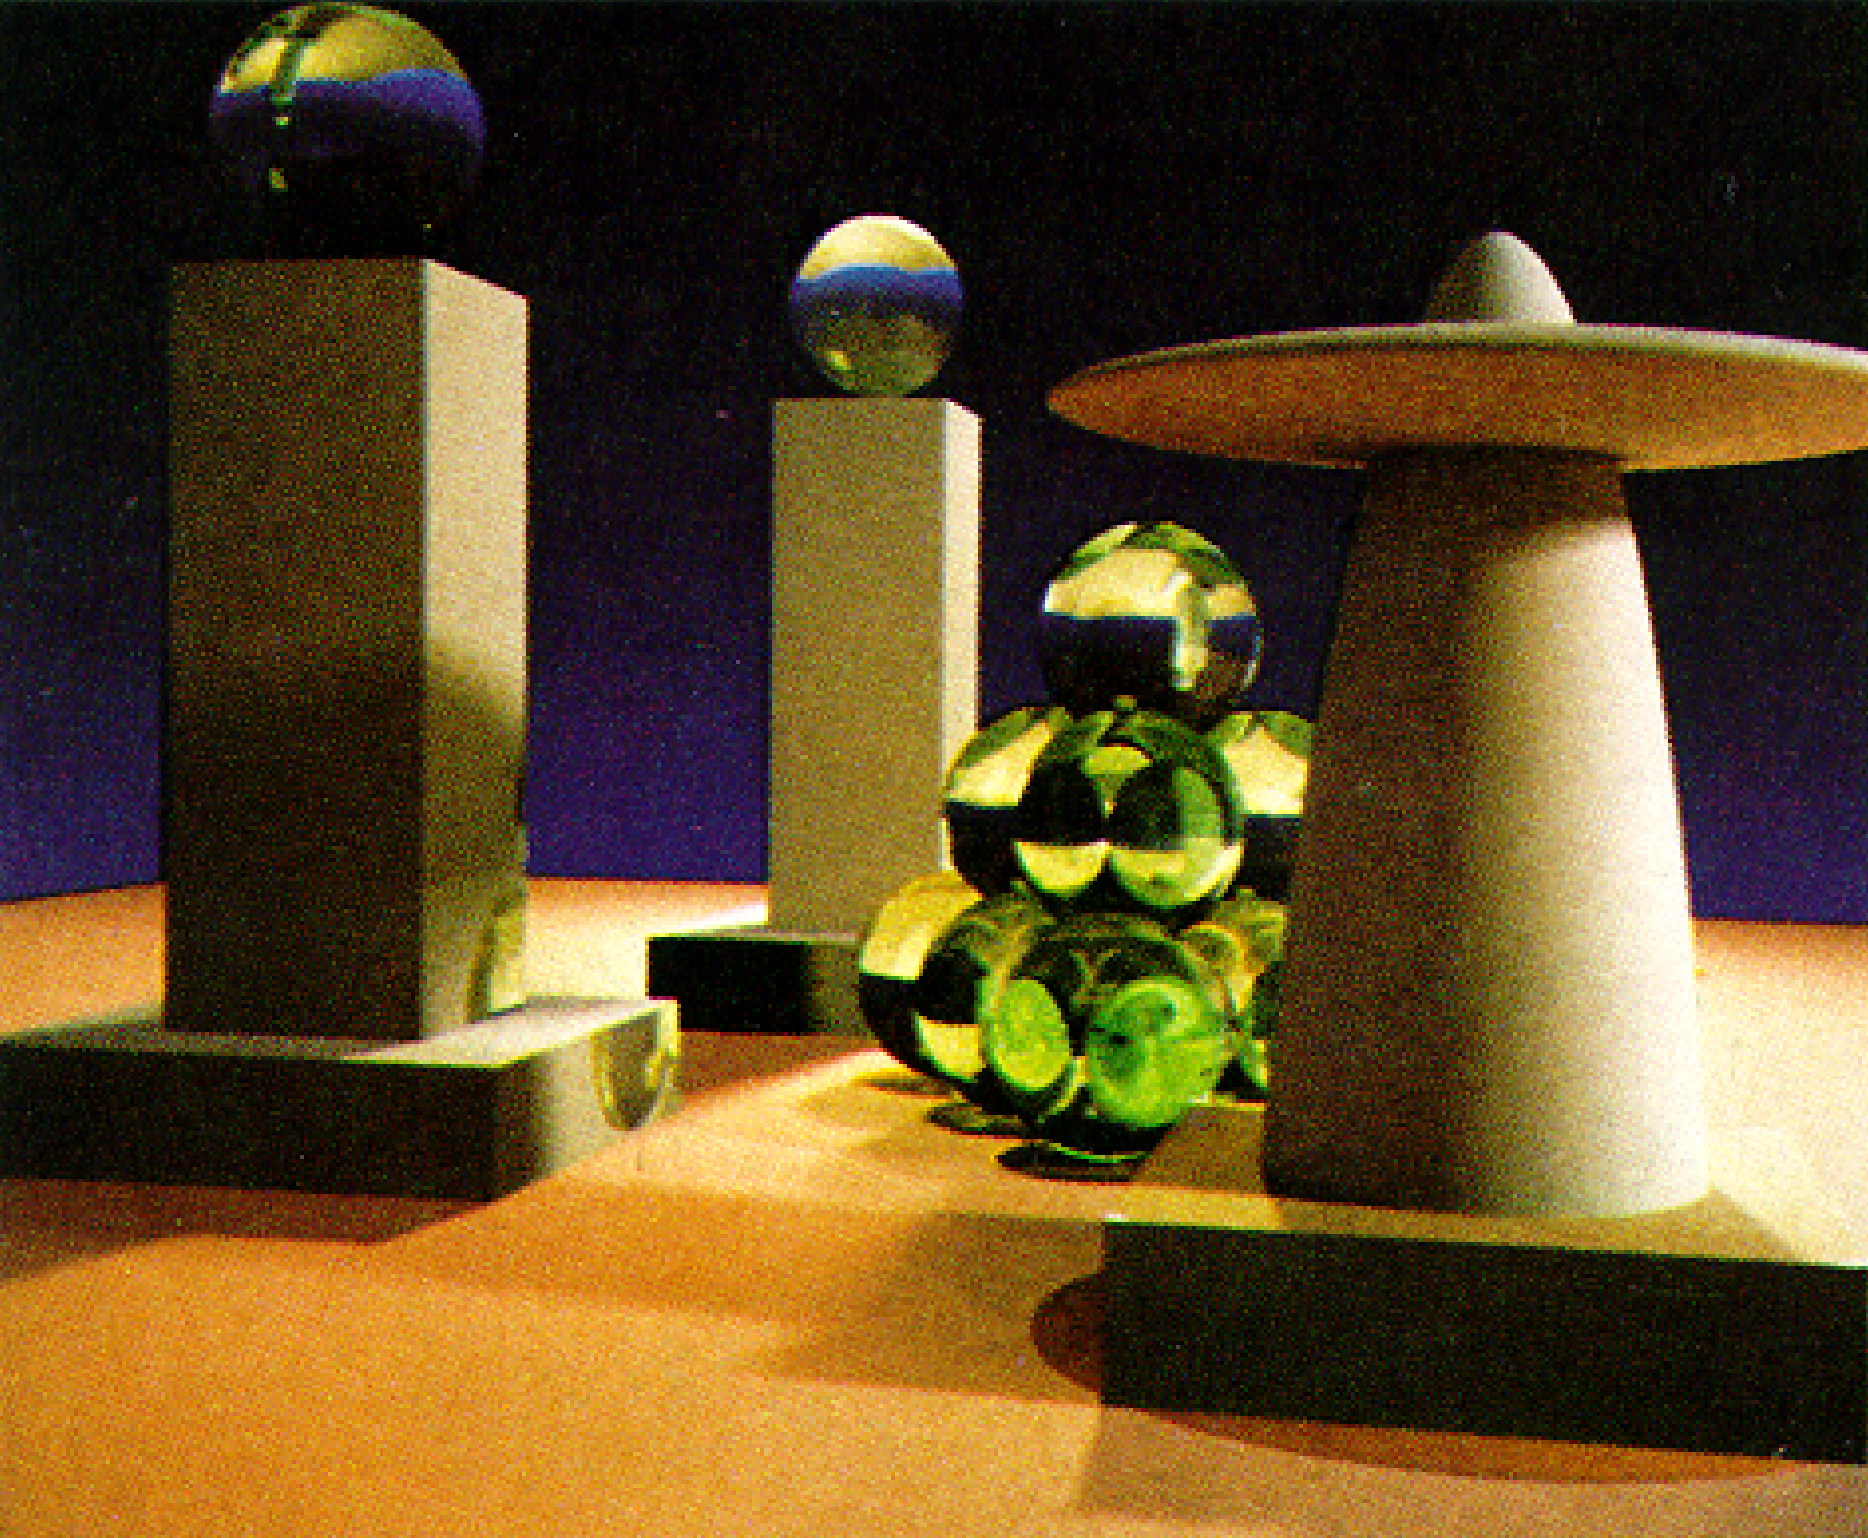
\includegraphics[height = 5.5cm]{rendering_equation_image.png}
    \caption{The image included in the original paper\cite{rendering_equation} that introduced path-tracing}
\end{figure}

The huge amount of existing rendering research can also be slightly frustrating once in a while, because it means it is difficult for me to devise novel algorithms. When implementing my renderer, there were quite a few times when a new idea of accelerating rendering emerged in my brain. In every occasion, a quick search on google scholar would lead to a well-written and in-depth paper that analyzes my ``novel'' proposal. As an example, I noticed that there're often regions of a rendered image that is significantly more noisy than other regions. Thus, I realized that if the renderer spend more time on these regions and less time in others, the quality of the image could improve with no extra cost. Of course, I soon discovered an ample amount of research that proposes all kinds of adaptive sampling strategies (e.g., \cite{rousselle2011adaptive}). 

Apart from the algorithmic side of rendering, this project also motivated me to put a lot of thought into writing well-structured and scalable code. The \texttt{Cavalry} renderer is designed so that new types of materials, geometries, and light sources and be added without any changes to the core path-tracing routine, and simultaneously, new variants of the path-tracing algorithm can be added without having to rewrite the code for these scene definition components. To achieve this kind of flexibility, the renderer underwent quite a few major refactors.

One observation that I made was that in some occasions, pursuing the scalability of the software sometimes means sacrificing performance or parallelizability. As an example, when organizing data, the array-of-structures pattern is often clearer and easier to modify, but the structure-of-arrays format enables better memory performance during parallelization. It was after many experiments when I settled into an architecture of the software that obtains a satisfying balance between these two aspects.

The completion of this project marks the end of 4 years of study at the computer science department of Oxford. Much like the project itself, my experience at Oxford had be delightfully challenging and extraordinarily rewarding. When I look back to the this project in the future, it will for sure be a pleasant reminder of the time I spent studying a field that I genuinely love.